\documentclass[12pt,a4paper,english]{article}
\usepackage [utf8]{inputenc}
\usepackage [english]{babel}
\usepackage [T1]{fontenc}
\usepackage {amsmath}
\usepackage{amsfonts}
\usepackage{amssymb}
\usepackage [top=3.4cm, bottom=2cm, left=3cm, right=3cm] {geometry}
\usepackage{setspace}
\usepackage{titlesec}
\usepackage{pgfkeys}
\usepackage{pgfgantt}
\setcounter{tocdepth}{3}
\usepackage{graphicx}
\usepackage{geometry}
\usetikzlibrary{positioning,shapes, shadows, arrows}
\usepackage{tikz}
\usepackage{url}
\linespread{1.3}
\usepackage{fancyhdr}
\pagestyle{fancyplain}
\fancyhead[L]{Paladim Milestone Assignment}
\fancyhead[C]{}
\fancyhead[R]{December 6 2013}

\usepackage{listings}

\begin{document}

\begin{titlepage}
    \vspace*{\fill}
    \begin{center}
      {\Huge Paladim Compiler}\\[0.7cm]
      {\large Alexander Worm Olsen - bdj816}\\[0.4cm]
      {\large Chi Dan Pham - vqr853}\\[0.4cm]
      {\large Troels Thompsen - qvw203}\\[0.4cm]
      {\small Group Project Milestone}\\[0.3cm]
      {\small December 6 2013}\\[0.3cm] 
      {\small Departmen of Computer Science}\\
      {\small University of Copenhagen}
    \end{center}
    \vspace*{\fill}
\end{titlepage}

\tableofcontents
\newpage
\section{Introduction}

For the milestone assignment we were asked to implement the grammar production rules for the paladim language, which is described in the groupproject description document.\\

In order to implement the grammar, we have edited the empty file \textit{Parser.grm}, which was already included in the source code handout. We also edited the \textit{Driver.sml} and the \textit{Lexer.lex} source code file, to use our new parser structure instead of the LL1Parser which was included in the handout. \\

For inspirational purposes we used the file \textit{example.pdf} which we found on absalon, and the groupproject description document. In these documents we found examples for creating type precedence, how to construct terminals and non-terminals, and how to use them correctly in the grammar.  \\

The following sections describe the changes made to each file respectively.

\section{Parser.grm}
\subsection{Definitions}
\subsubsection{Terminals}
The first definition in the parser, is the definition of terminals, which in mosmlyac is called tokens.

\begin{figure}[h]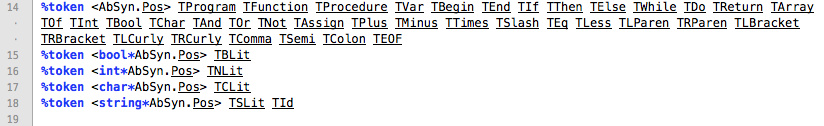
\includegraphics[width=15cm]{Token.jpg}\caption{Parser.grm Tokens}\end{figure}
Here we use the abstract syntax type definitions to define the types of our tokens. The tokens themselves are defined in the \textit{Lexer.lex} file. We simply found all tokens in the lexer, and defined tokens for them.

\subsubsection{Precedence Rules}

Next we define our precedence rules, to prevent shift / reduce conflicts. The rules at the bottom take the highest precedence.

\begin{figure}[h]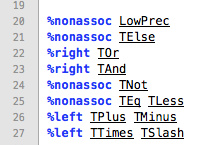
\includegraphics[]{Prec.jpg}\caption{Parser.grm Precedence}\end{figure}
We use left associative precedence for arithmetic operations, ranking \textit{TTimes} and \textit{TSlash} higher than \textit{TPlus} and \textit{TMinus}. \\

We define comparison operations \textit{TLess} and \textit{TEq} as non-associative, since it is not specified whether comparison is associative in Paladim in the project description. \\

The logical operation \textit{TNot} is defined as non-associative because it is unary. We define the other logical operations \textit{TAnd} and \textit{TOr} as left-associative (they can be either left- or right-associative, but should not be non-associative). Here \textit{TNot} takes precedence over \textit{TAnd} which takes precedence over \textit{TOr}. \\

The last two precedence rules are defined to resolve the shift / reduce conflict, which occurs when trying to write productions for If-Then-Else and If-Then. This conflict occurs in the following scenario. 
\begin{lstlisting}
if a > b then
    if c = d then
        return a
    else
        return b
\end{lstlisting}
In this scenario the parser does not know whether to match the production for If-Then-Else, or the production for If-Then. If it shifts, the else belongs to the inner if-statement, but if it reduces, the else belongs to the outer if-statement. In this scenario, we actually always wants to shift, because the else should belong to the closest previous if-then-statement. In order to accomplish this, we define TElse to take precedence over "LowPrec". We later assign "LowPrec" to the If-Then production grammar, and thus resolve the shift / reduce conflict.

\subsubsection{Non-Terminals}

In this section we define our start symbol, and the non-terminals for our productions. \\
\begin{figure}[h]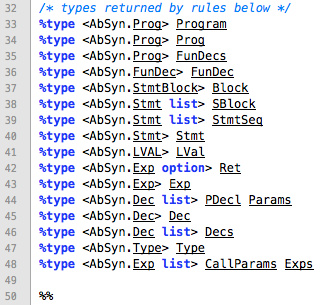
\includegraphics[]{Types.jpg}\caption{Parser.grm}\end{figure}
The types used for the non-terminals are defined in \textit{AbSyn.sml}. The actual non-terminals are defined in figure 3 in the group project definition document. The start symbol "Program" was defined by us, in order to handle end of file.

\pagebreak
\subsection{Grammar}

In this section we define the grammar used by the parser. For easier analysis we have divided the grammar into sections.
In general we built the grammar by looking at the production definitions in figure 3 in the group project definition. The type we return in the productions, are defined in the \textit{AbSyn.sml}. 

\subsubsection{Program structure}

\begin{figure}[h]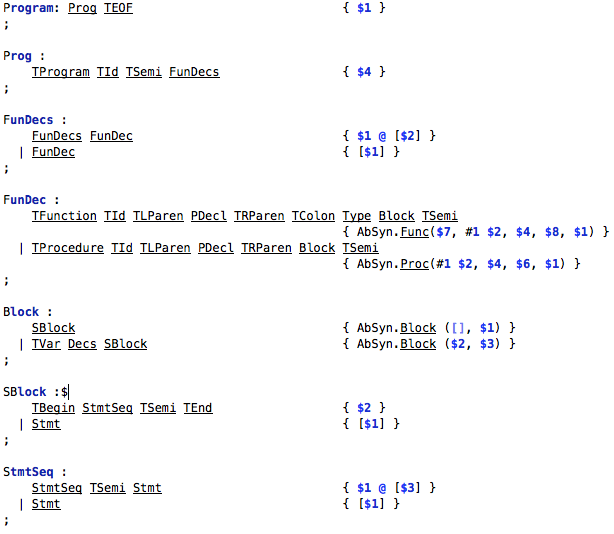
\includegraphics[width=15cm]{program_structure.png}\caption{Parser.grm}\end{figure}
The most important change in this section, is the Block production. To begin with we had a DBlock production, as described in figure 3 in the group project definition. This caused a shift / reduce conflict, which we resolved by combining the DBlock with the Block production. 

\pagebreak

\subsubsection{Statements, Values and Expressions}

\begin{figure}[h]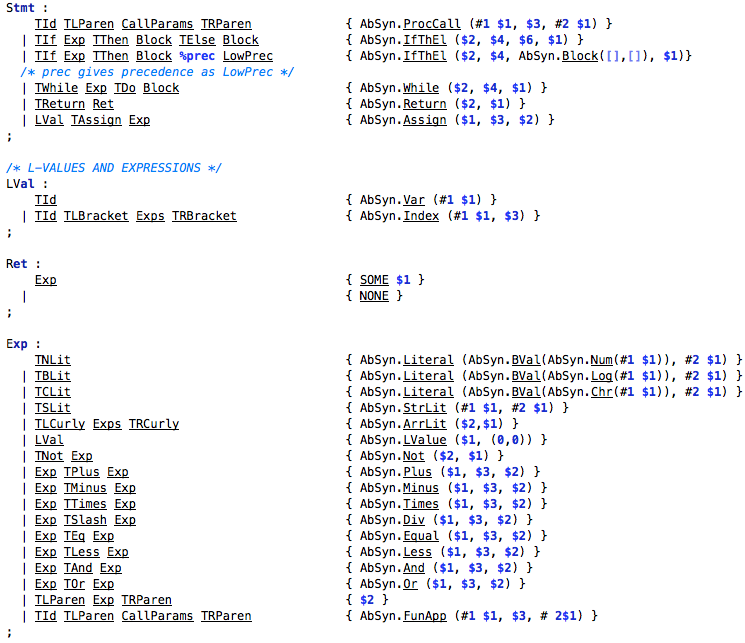
\includegraphics[width=16cm]{statements.png}\caption{Parser.grm}\end{figure}
The most important change in this section, is the \textit{TIf Exp TThen Block \%prec LowPrec} production. As described in the non-terminal definitions, we need to assign lower precedence to the If-Then production. This is done by adding \%prec LowPrec at the end of the production. \

\textbf{The Exp LVal production} in this section might be problematic. This production needs to return an AbSyn.LValue(LVal, Pos). However this is not possible, because we call another production which only returns an LVal without a position, therefore we just pass (0,0) on.

\subsubsection{Parameters and Procedures}
At the end we have our simple definitions for parameters and declarations.
\begin{figure}[h]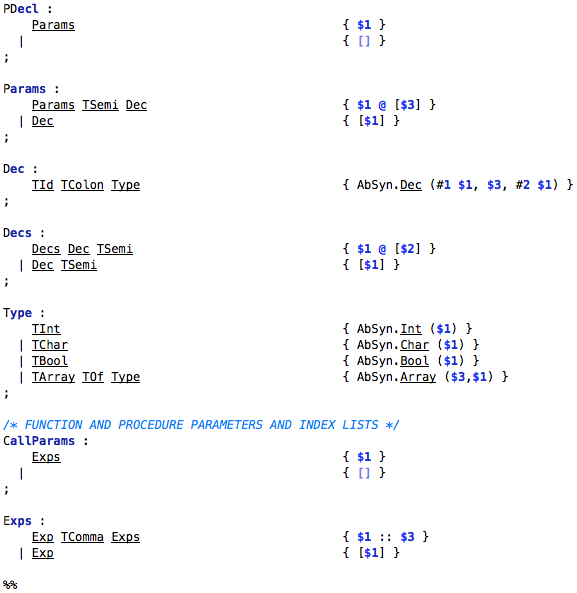
\includegraphics[width=15cm]{params.png}\caption{Parser.grm}\end{figure}

\newpage
\subsection{Driver.sml}
In the driver file we have uncommented the two lines which was meant for the LL1 parser and instead inserted the appropriate ones for our parser (line 57 and 69). Furthermore we have uncommented the Parser.ParseError, because this error message will be caught by the Parsing.ParseError, and instead only created compile errors. These changed are shown in figure 7.
\begin{figure}[h]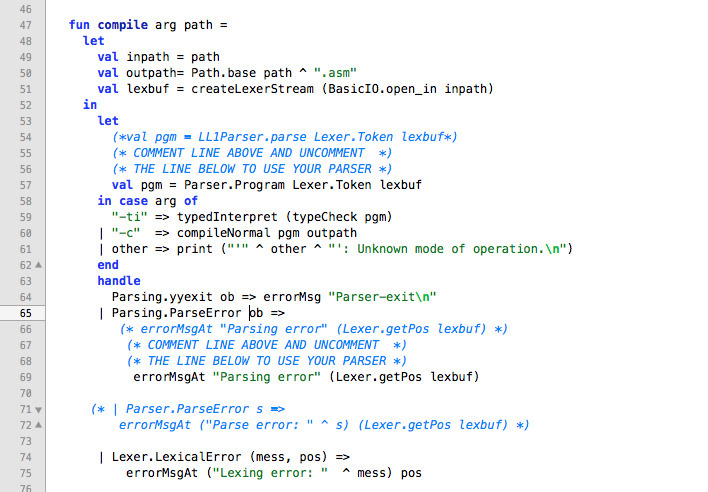
\includegraphics[width=15cm]{driver.jpg}\caption{Driver.sml}\end{figure}

\subsection{Lexer.lex}
In the \textit{Lexer.lex} we have changed all instances of LL1parser to Parser, thereby including our newly created Parser.grm instead of the handout. Please note that this code is left out.

\subsection{Functionality of multiplication}
As task 2 stated we were to implement the functionality of multiplication, division, OR and NOT in the parser. These operations have not been implemented in the rest of the compiler, so in order to test our implementation of arithmetic precedence, we implemented multiplication. This included changes to the following files: \textit{Compiler.sml},
\textit{TpInterpret.sml},\textit{Type.sml},\textit{TpAbSyn.sml}.
\begin{figure}\includegraphics[width=15cm]{compiler.jpg} \caption{Compile.sml}\end{figure}
\begin{figure}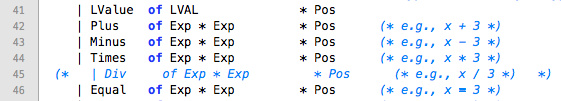
\includegraphics[width=15cm, height = 2cm]{TpAbSyn1.jpg}\caption{TpAbSyn.sml}\end{figure}
\begin{figure}
\includegraphics[width=15cm]{TpAbSyn2.jpg}\caption{TpAbSyn.sml}\end{figure}
\begin{figure}
\includegraphics[]{TpAbSyn3.jpg}\caption{TpAbSyn.sml}\end{figure}
\begin{figure}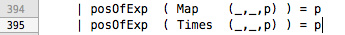
\includegraphics[]{TpAbSyn4.jpg}\caption{TpAbSyn.sml}\end{figure}
\begin{figure}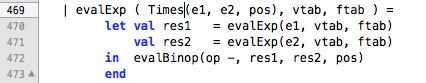
\includegraphics[]{TpInterpret.jpg}\caption{TpInterpret.sml}\end{figure}
\begin{figure}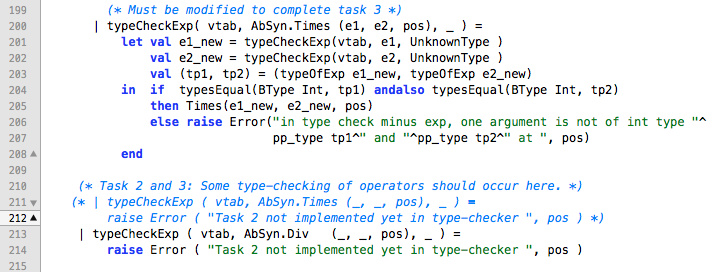
\includegraphics[width=15cm]{Type.jpg}\caption{Type.sml}\end{figure}

\newpage
\section{Testing}
We have made two test examples; one that covers the problem with nested \textit{if then else} and another one that tests precedence with multiplication and addition. We ran the compiled programs in Mars and they returned the expected results ("If-then-else virker!!!" and "det virker jo").
\begin{figure}[h]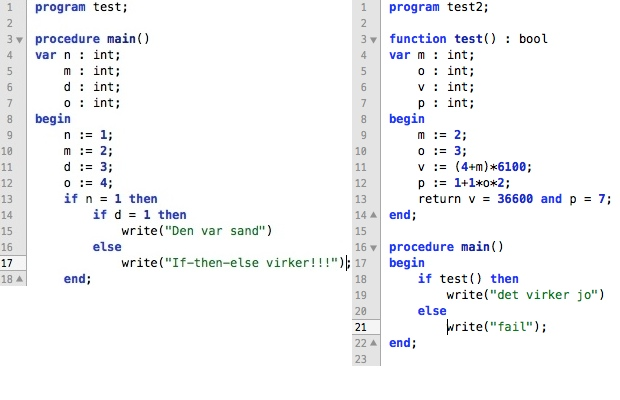
\includegraphics[height=10cm]{Testing.jpg}\caption{Test.pal og Test2.pal}\end{figure}















\end{document}\